\documentclass[../main.tex]{subfiles}
\begin{document}

% En compilation individuelle, la mention légale est affichée.
% Dans le livre complet, elle figure déjà sur la page de garde.
\ifSubfilesClassLoaded{\PageLegaleChapitre}{}

\chapter{Produits remarquables et factorisation}
\label{chap:produits-remarquables}

% =====================================================
\section{Les produits remarquables}
% =====================================================

Un produit remarquable est une formule qui permet de développer rapidement certains produits sans passer par la double distributivité terme à terme.

\subsection{Les trois formules fondamentales}

\begin{propriete}[Produits remarquables]
Quels que soient les réels $a$ et $b$ :
\begin{enumerate}[label=\textbf{(\arabic*)}]
  \item \textbf{Carré d'une somme :} $(a + b)^2 = a^2 + 2ab + b^2$
  \item \textbf{Carré d'une différence :} $(a - b)^2 = a^2 - 2ab + b^2$
  \item \textbf{Produit de la somme par la différence :} $(a + b)(a - b) = a^2 - b^2$
\end{enumerate}
\end{propriete}

\subsection{Illustration géométrique du carré d'une somme}

Pour comprendre pourquoi $(a+b)^2 = a^2 + 2ab + b^2$, on calcule l'aire d'un grand carré de côté $(a+b)$ :

\begin{center}
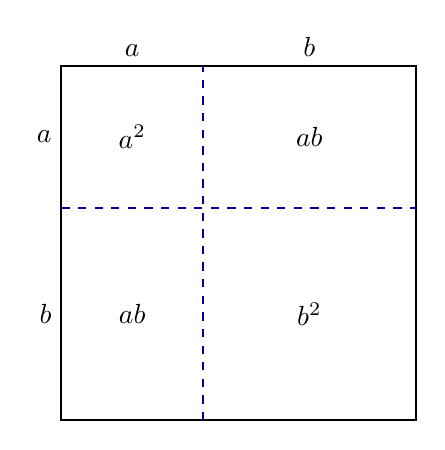
\begin{tikzpicture}[scale=0.9]
  % Grand carré
  \draw[thick] (0,0) rectangle (5,5);
  \draw[dashed, thick, blue!60!black] (2,0) -- (2,5);
  \draw[dashed, thick, blue!60!black] (0,3) -- (5,3);

  % Aires intérieures
  \node at (1,4) {$a^2$};
  \node at (3.5,4) {$ab$};
  \node at (1,1.5) {$ab$};
  \node at (3.5,1.5) {$b^2$};

  % Dimensions extérieures
  \node[above] at (1,5) {$a$};
  \node[above] at (3.5,5) {$b$};
  \node[left] at (0,4) {$a$};
  \node[left] at (0,1.5) {$b$};
\end{tikzpicture}
\end{center}

L'aire totale est la somme des quatre aires intérieures : $a^2 + ab + ab + b^2 = a^2 + 2ab + b^2$.

\textbf{Exemples.}
\begin{itemize}
  \item $(x + 3)^2 = x^2 + 2 \times x \times 3 + 3^2 = x^2 + 6x + 9$
  \item $(2x - 5)^2 = (2x)^2 - 2 \times (2x) \times 5 + 5^2 = 4x^2 - 20x + 25$
  \item $(4x - 3)(4x + 3) = (4x)^2 - 3^2 = 16x^2 - 9$
\end{itemize}

\begin{attention}
L'erreur classique :
\[
(a + b)^2 \neq a^2 + b^2 \qquad\text{et}\qquad (a - b)^2 \neq a^2 - b^2.
\]
Il manque toujours le double produit ($2ab$ ou $-2ab$) au milieu.
\end{attention}

\subsection{Application au calcul mental}

Les produits remarquables permettent de calculer sans calculatrice :
\[
101^2 = (100+1)^2 = 10\,000 + 200 + 1 = 10\,201, \qquad
49 \times 51 = (50-1)(50+1) = 2\,500 - 1 = 2\,499.
\]

% =====================================================
\section{La factorisation}
% =====================================================

Factoriser une expression, c'est la transformer d'une \textbf{somme} (ou d'une différence) en un \textbf{produit} de facteurs. C'est l'opération inverse du développement.

\subsection{Méthode 1 : la mise en évidence}

\begin{methode}
\begin{enumerate}
  \item Chercher un facteur commun (nombre, lettre ou parenthèse) présent dans tous les termes.
  \item Le mettre en évidence en utilisant la distributivité à l'envers : $ka + kb = k(a + b)$.
\end{enumerate}
\end{methode}

\textbf{Exemples.}
\begin{itemize}
  \item $5x^2 - 10x = 5x(x - 2)$
  \item $3x(x+1) - 4(x+1) = (x+1)(3x - 4)$
\end{itemize}

\subsection{Méthode 2 : utiliser les produits remarquables}

On lit les identités remarquables \textbf{de droite à gauche} :
\begin{enumerate}
  \item $a^2 + 2ab + b^2 = (a + b)^2$
  \item $a^2 - 2ab + b^2 = (a - b)^2$
  \item $a^2 - b^2 = (a + b)(a - b)$
\end{enumerate}

\textbf{Exemples.}
\begin{itemize}
  \item $x^2 + 8x + 16 = x^2 + 2 \times x \times 4 + 4^2 = (x + 4)^2$
  \item $9x^2 - 25 = (3x)^2 - 5^2 = (3x - 5)(3x + 5)$
\end{itemize}

\begin{attention}
Une somme de deux carrés, comme $x^2 + 9$, ne se factorise pas avec ces formules.
\end{attention}

% =====================================================
\section{Récapitulatif}
% =====================================================

\begin{tcolorbox}[colback=gray!6,colframe=gray!60!black,title={\bfseries À retenir}]
\textbf{Développer} : transformer un produit en somme. \quad \textbf{Factoriser} : transformer une somme en produit.
\[
(a+b)^2 = a^2 + 2ab + b^2, \qquad (a-b)^2 = a^2 - 2ab + b^2, \qquad (a+b)(a-b) = a^2 - b^2.
\]
\textbf{Réflexes :} ne jamais oublier le double produit~; en factorisation, chercher d'abord un facteur commun, puis reconnaître un produit remarquable.
\end{tcolorbox}

\newpage
% =====================================================
\section{Exercices}
% =====================================================

\subsection{Série A -- Briefing au sol : développer}

\begin{enumerate}[label=\textbf{\arabic*.}]

\item Développe et réduis :
\begin{enumerate}[label=\alph*)]
  \item $(x + 4)^2$ \qquad
  \item $(3x - 1)^2$ \qquad
  \item $(5 + 2x)^2$ \qquad
  \item $(x - 7)(x + 7)$
  \item $(2x - 3)(2x + 3)$ \qquad
  \item $(-x + 4)^2$ \qquad
  \item $(3x - 2)^2 - (x+1)$ \quad\textit{(attention aux signes !)}
\end{enumerate}

\end{enumerate}

\subsection{Série B -- Carnet de campagne : factoriser par mise en évidence}

\begin{enumerate}[label=\textbf{\arabic*.},start=2]

\item Factorise le plus possible :
\begin{enumerate}[label=\alph*)]
  \item $3x^2 + 12x$ \qquad
  \item $7x^3 - 14x^2 + 21x$ \qquad
  \item $a(x - 2) + b(x - 2)$ \qquad
  \item $4x(2x - 1) - 3(2x - 1)$
\end{enumerate}

\end{enumerate}

\subsection{Série C -- Factoriser avec les produits remarquables}

\begin{enumerate}[label=\textbf{\arabic*.},start=3]

\item Factorise en reconnaissant un produit remarquable :
\begin{enumerate}[label=\alph*)]
  \item $x^2 + 10x + 25$ \qquad
  \item $x^2 - 9$ \qquad
  \item $4x^2 - 12x + 9$ \qquad
  \item $16x^2 - 49$ \qquad
  \item $x^2 - 2x + 1$
\end{enumerate}

\end{enumerate}

\subsection{Série D -- Missions de vol et de camp}

\textbf{Mission 1 -- Terrain de camp.}
La troupe dispose d'un terrain carré de côté $x$ (en mètres). Elle l'agrandit de $3$ m sur chaque côté : le nouveau terrain est un carré de côté $x + 3$.
\begin{enumerate}[label=\alph*)]
  \item Exprime l'aire du nouveau terrain et développe-la.
  \item De combien l'aire a-t-elle augmenté ? Simplifie l'expression.
\end{enumerate}

\textbf{Mission 2 -- Calcul mental du copilote.}
Sans calculatrice, à l'aide d'un produit remarquable :
\begin{enumerate}[label=\alph*)]
  \item $101^2$ \qquad
  \item $99^2$ \qquad
  \item $52 \times 48$ \qquad
  \item $1\,003 \times 997$
\end{enumerate}

\textbf{Mission 3 -- Le tarmac.}
Une aire de stationnement rectangulaire mesure $(x+5)$ m sur $(x-5)$ m.
\begin{enumerate}[label=\alph*)]
  \item Montre que son aire vaut $x^2 - 25$.
  \item Calcule l'aire pour $x = 45$.
\end{enumerate}

\textbf{Mission 4 -- Le camp et sa clairière.}
Un terrain carré de côté $a$ contient en son centre une clairière carrée de côté $b$ (avec $a > b$). La zone boisée est la partie restante.
\begin{enumerate}[label=\alph*)]
  \item Exprime l'aire de la zone boisée, puis factorise-la.
  \item Calcule cette aire pour $a = 13$ m et $b = 7$ m, sans calculatrice.
\end{enumerate}

\subsection{Défi bonus}

\begin{enumerate}[label=\alph*)]
  \item Développe $(x + 1)^3$ en utilisant $(x+1)^2(x+1)$.
  \item Factorise $2x^3 - 18x$ en deux étapes (mise en évidence, puis produit remarquable).
\end{enumerate}

\newpage
% =====================================================
\section{Corrigés}
% =====================================================

\subsection*{Série A}

\textbf{1.} a) $x^2 + 8x + 16$ \quad b) $9x^2 - 6x + 1$ \quad c) $25 + 20x + 4x^2$ \quad d) $x^2 - 49$ \quad e) $4x^2 - 9$ \quad f) $x^2 - 8x + 16$ \quad g) $(9x^2 - 12x + 4) - (x + 1) = 9x^2 - 13x + 3$

\subsection*{Série B}

\textbf{2.} a) $3x(x + 4)$ \quad b) $7x(x^2 - 2x + 3)$ \quad c) $(x - 2)(a + b)$ \quad d) $(2x - 1)(4x - 3)$

\subsection*{Série C}

\textbf{3.} a) $(x + 5)^2$ \quad b) $(x - 3)(x + 3)$ \quad c) $(2x - 3)^2$ \quad d) $(4x - 7)(4x + 7)$ \quad e) $(x - 1)^2$

\subsection*{Série D}

\textbf{Mission 1.}
a) $(x+3)^2 = x^2 + 6x + 9$.
b) Augmentation : $(x+3)^2 - x^2 = 6x + 9$ m\textsuperscript{2}.

\textbf{Mission 2.}
a) $(100+1)^2 = 10\,201$ \quad
b) $(100-1)^2 = 10\,000 - 200 + 1 = 9\,801$ \quad
c) $(50+2)(50-2) = 2\,500 - 4 = 2\,496$ \quad
d) $(1\,000+3)(1\,000-3) = 1\,000\,000 - 9 = 999\,991$

\textbf{Mission 3.}
a) $(x+5)(x-5) = x^2 - 25$.
b) $45^2 - 25 = 2\,025 - 25 = 2\,000$ m\textsuperscript{2}.

\textbf{Mission 4.}
a) $a^2 - b^2 = (a-b)(a+b)$.
b) $(13-7)(13+7) = 6 \times 20 = 120$ m\textsuperscript{2} (vérification : $169 - 49 = 120$).

\subsection*{Défi bonus}

a) $(x^2 + 2x + 1)(x+1) = x^3 + 3x^2 + 3x + 1$.

b) $2x^3 - 18x = 2x(x^2 - 9) = 2x(x - 3)(x + 3)$.

\end{document}
